\documentclass{article}

\usepackage{times}
\usepackage{geometry}
\geometry{a4paper,left=0.6cm,right=0.7cm,top=1cm,bottom=1cm,columnsep=0.8cm}

\usepackage{fontawesome}
\usepackage[hidelinks]{hyperref}
\usepackage{multicol,paracol,tikz,hyphsubst,moresize,hyphenat,adjustbox,tabularx,xcolor,enumitem}
\newcolumntype{Y}{>{\RaggedRight\arraybackslash}X}
\setlist[itemize]{itemsep=1pt,leftmargin=*,topsep=-10pt}

\definecolor{maincolor}{HTML}{ffffff}
\definecolor{seccolor}{HTML}{0b1f3b}
\definecolor{gray}{HTML}{8c94a9}
\definecolor{sidetext}{HTML}{59cee5}
\definecolor{Green}{HTML}{2caf00}
\definecolor{lightgray}{HTML}{D3D3D3}

% --- bande latérale bleue
\usepackage{eso-pic}
\AddToShipoutPictureBG{%
  \begin{tikzpicture}[remember picture,overlay]
    \fill[seccolor] (0.7\paperwidth,0) rectangle (\paperwidth,\paperheight);
    \fill[maincolor] (0,0) rectangle (0.7\paperwidth,\paperheight);
  \end{tikzpicture}%
}

\setlength{\parindent}{0pt}
\newcommand{\cvsection}[1]{%
  \setlength{\arrayrulewidth}{2pt}
  \begin{tabular}{@{}ll}
  \textbf{\Large #1}\\ \hline
  \end{tabular}\vspace{4pt}
}

\newcommand*{\ClipSep}{0.4cm}

% ------------------------------------------------------------------
\begin{document}\pagestyle{empty}
\columnratio{0.7}\begin{paracol}{2}

% --------- colonne gauche -----------------------------------------
\begin{minipage}{0.7\linewidth}
{\LARGE\textbf{Pape Saliou FALL}}

\bigskip
{\large\textbf{Ingénieur Data Scientist \& Développeur IA}}
\end{minipage}\hfill
\begin{minipage}{0.18\linewidth}
\begin{tikzpicture}
\node[inner sep=0pt]{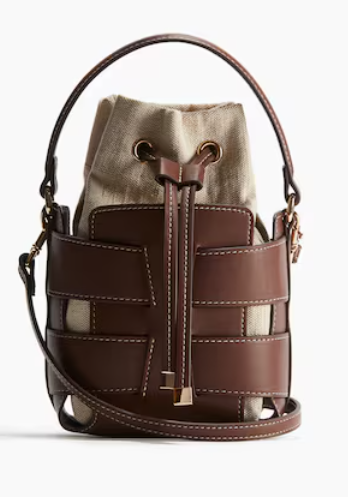
\includegraphics[width=\linewidth]{e573c65c6e8343ff84046454c7b480fc.png}};
\draw[white,rounded corners=\ClipSep,line width=\ClipSep]
      (current bounding box.north west) --
      (current bounding box.north east) --
      (current bounding box.south east) --
      (current bounding box.south west) -- cycle;
\end{tikzpicture}
\end{minipage}

\cvsection{Profil}
Data Scientist et développeur IA avec une solide formation en analyse statistique et en apprentissage automatique. J’exploite Python et des frameworks de deep learning pour transformer des données hétérogènes en solutions concrètes. Autonome tout en appréciant le travail d’équipe, j’ai mené des projets de plateformes IA et d’automatisation de processus métier. Je recherche un environnement innovant où relever de nouveaux défis et générer de la valeur à partir des données.

\cvsection{EXPÉRIENCE}

\colorbox{maincolor}{%
  \begin{minipage}{\linewidth}
    \textbf{Data Scientist \& Développeur IA} \\ Prepaya \\ janv. 2024 – Présent
    \begin{itemize}
      \item Développé une plateforme IA full-stack (Python/JavaScript, Flask) déployée sur Heroku avec PostgreSQL. \item Réalisé des analyses de séries chronologiques et mis en place des modèles ML \& deep learning via Scikit-learn, Tensorflow et Keras. \item Intégré l’API OpenAI pour automatiser la génération d’insights et enrichir les fonctionnalités produit.
    \end{itemize}
  \end{minipage}}

\vspace{3mm}


\colorbox{maincolor}{%
  \begin{minipage}{\linewidth}
    \textbf{Apprenti Risk Analyst \& Data Scientist} \\ AXA XL (Groupe AXA) \\ déc. 2022 – déc. 2023
    \begin{itemize}
      \item Automatisé la collecte des données financières à l’aide de Python et VBA pour fiabiliser les reportings. \item Conçu des tableaux de bord Power BI facilitant le suivi de la facturation pour les équipes finance et management. \item Développé des applications prédictives estimant la probabilité de sinistre à partir des historiques clients.
    \end{itemize}
  \end{minipage}}

\vspace{3mm}


\colorbox{maincolor}{%
  \begin{minipage}{\linewidth}
    \textbf{Apprenti Data Scientist} \\ Prepaya \\ sept. 2021 – août 2022
    \begin{itemize}
      \item Appliqué des modèles de deep learning NLP (BERT, T5) pour générer automatiquement des formulaires. \item Réalisé une analyse de sentiment sur les retours clients afin d’améliorer la satisfaction et les process internes. \item Automatisé la collecte de données web avec Python (BeautifulSoup, Selenium) et documenté les livrables sous LaTeX.
    \end{itemize}
  \end{minipage}}

\cvsection{FORMATION}

    \begin{tabularx}{\linewidth}{@{}c X@{}}
    \textcolor{sidetext}{\faGraduationCap} &
    \textbf{Master 2 Data Science} \\
    & Sorbonne Université \\
    & \begin{itemize}[leftmargin=*]
  \item Analyse de données, séries chronologiques et apprentissage statistique appliqué. \item Machine learning, deep learning et modèles de structure latente. \item Bases de données, calcul parallèle et projets pratiques en équipe.
\end{itemize} \\
    & \textit{sept. 2021 – mars 2022}
    \end{tabularx}
    

% --------- colonne droite (bleue) ---------------------------------
\switchcolumn\color{white}\hspace*{0.4cm}\begin{minipage}{0.88\linewidth}

\cvsection{CONTACT}
\begin{tabular}{@{}c l}
  \faPhone & \href{tel:0753481453}{0753481453} \\[2pt]
  \faEnvelope & \href{mailto:papesalioufall2@gmail.com}{papesalioufall2@gmail.com} \\[2pt]
  \faMapMarker & 95300 Pontoise\\ \\[2pt]
  \faLinkedin & \href{pape-saliou-fall-43154a211}{pape-saliou-fall-43154a211}
\end{tabular}

\cvsection{COMPÉTENCES}

\begin{itemize}[leftmargin=*]
\item Python
\item R
\item SQL
\item JavaScript
\item C++
\item Tensorflow
\item PowerBI\end{itemize}


\cvsection{LANGUES}
\begin{itemize}[leftmargin=*]
\item Français - \textcolor{gray}{Natif}
\item Anglais - \textcolor{gray}{B2}\end{itemize}

\cvsection{CENTRES D’INTÉRÊT}
\begin{itemize}[leftmargin=*]
\item Football
\item Natation
\item Lecture
\item Poésie
\end{itemize}

\end{minipage}
\end{paracol}
\end{document}
